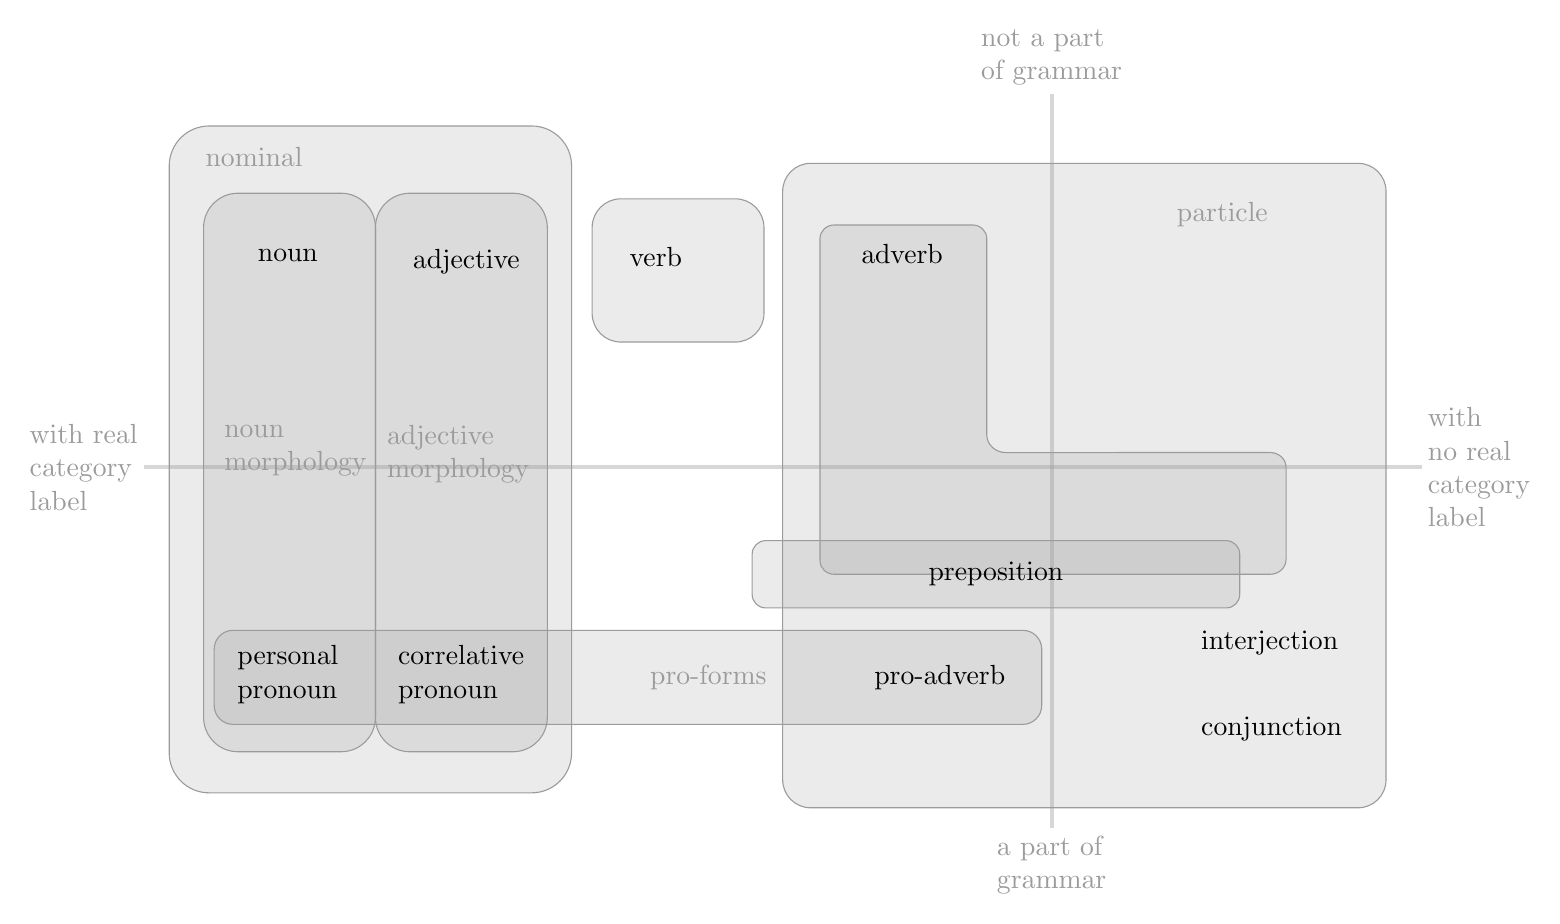
\begin{tikzpicture}[x=0.75pt,y=0.75pt,yscale=-0.9,xscale=0.9]
    %uncomment if require: \path (0,674); %set diagram left start at 0, and has height of 674
    
    %Straight Lines [id:da0819119912251447] 
    \draw [color={rgb, 255:red, 155; green, 155; blue, 155 }  ,draw opacity=0.4 ][line width=1.5]    (109.33,384.91) -- (793.33,384.91) ;
    %Rounded Rect [id:dp9835773367494156] 
    \draw  [color={rgb, 255:red, 155; green, 155; blue, 155 }  ,draw opacity=1 ][fill={rgb, 255:red, 155; green, 155; blue, 155 }  ,fill opacity=0.2 ] (141.33,256.64) .. controls (141.33,246.48) and (149.57,238.24) .. (159.73,238.24) -- (214.93,238.24) .. controls (225.1,238.24) and (233.33,246.48) .. (233.33,256.64) -- (233.33,518.84) .. controls (233.33,529) and (225.1,537.24) .. (214.93,537.24) -- (159.73,537.24) .. controls (149.57,537.24) and (141.33,529) .. (141.33,518.84) -- cycle ;
    %Rounded Rect [id:dp12690257166641228] 
    \draw  [color={rgb, 255:red, 155; green, 155; blue, 155 }  ,draw opacity=1 ][fill={rgb, 255:red, 155; green, 155; blue, 155 }  ,fill opacity=0.2 ] (233.33,256.64) .. controls (233.33,246.48) and (241.57,238.24) .. (251.73,238.24) -- (306.93,238.24) .. controls (317.1,238.24) and (325.33,246.48) .. (325.33,256.64) -- (325.33,518.84) .. controls (325.33,529) and (317.1,537.24) .. (306.93,537.24) -- (251.73,537.24) .. controls (241.57,537.24) and (233.33,529) .. (233.33,518.84) -- cycle ;
    %Rounded Rect [id:dp4571683339095527] 
    \draw  [color={rgb, 255:red, 155; green, 155; blue, 155 }  ,draw opacity=1 ][fill={rgb, 255:red, 155; green, 155; blue, 155 }  ,fill opacity=0.2 ] (349.33,256.57) .. controls (349.33,248.1) and (356.2,241.24) .. (364.67,241.24) -- (426,241.24) .. controls (434.47,241.24) and (441.33,248.1) .. (441.33,256.57) -- (441.33,302.57) .. controls (441.33,311.04) and (434.47,317.91) .. (426,317.91) -- (364.67,317.91) .. controls (356.2,317.91) and (349.33,311.04) .. (349.33,302.57) -- cycle ;
    %Rounded Rect [id:dp13945556495695044] 
    \draw  [color={rgb, 255:red, 155; green, 155; blue, 155 }  ,draw opacity=1 ][fill={rgb, 255:red, 155; green, 155; blue, 155 }  ,fill opacity=0.2 ] (122.93,223.64) .. controls (122.93,211.82) and (132.51,202.24) .. (144.33,202.24) -- (316.93,202.24) .. controls (328.75,202.24) and (338.33,211.82) .. (338.33,223.64) -- (338.33,537.84) .. controls (338.33,549.66) and (328.75,559.24) .. (316.93,559.24) -- (144.33,559.24) .. controls (132.51,559.24) and (122.93,549.66) .. (122.93,537.84) -- cycle ;
    %Straight Lines [id:da9866800561526903] 
    \draw [color={rgb, 255:red, 155; green, 155; blue, 155 }  ,draw opacity=0.4 ][line width=1.5]    (595.33,577.91) -- (595.33,184.91) ;
    %Rounded Rect [id:dp9919662328975185] 
    \draw  [color={rgb, 255:red, 155; green, 155; blue, 155 }  ,draw opacity=1 ][fill={rgb, 255:red, 155; green, 155; blue, 155 }  ,fill opacity=0.2 ] (435,431.44) .. controls (435,427.46) and (438.22,424.24) .. (442.2,424.24) -- (688.8,424.24) .. controls (692.78,424.24) and (696,427.46) .. (696,431.44) -- (696,453.04) .. controls (696,457.02) and (692.78,460.24) .. (688.8,460.24) -- (442.2,460.24) .. controls (438.22,460.24) and (435,457.02) .. (435,453.04) -- cycle ;
    %Rounded Rect [id:dp04492990660366303] 
    \draw  [color={rgb, 255:red, 155; green, 155; blue, 155 }  ,draw opacity=1 ][fill={rgb, 255:red, 155; green, 155; blue, 155 }  ,fill opacity=0.2 ] (147,482.31) .. controls (147,476.75) and (151.51,472.24) .. (157.07,472.24) -- (579.93,472.24) .. controls (585.49,472.24) and (590,476.75) .. (590,482.31) -- (590,512.51) .. controls (590,518.07) and (585.49,522.57) .. (579.93,522.57) -- (157.07,522.57) .. controls (151.51,522.57) and (147,518.07) .. (147,512.51) -- cycle ;
    %Shape: Path Data [id:dp3209513602067542] 
    \draw  [color={rgb, 255:red, 155; green, 155; blue, 155 }  ,draw opacity=1 ][fill={rgb, 255:red, 155; green, 155; blue, 155 }  ,fill opacity=0.2 ] (478.97,255.24) -- (552.94,255.24) .. controls (557.16,255.24) and (560.58,258.46) .. (560.58,262.43) -- (560.58,367.51) .. controls (560.58,372.79) and (565.13,377.07) .. (570.74,377.07) -- (630.37,377.07) .. controls (630.59,377.07) and (630.82,377.07) .. (631.04,377.05) -- (712.31,377.05) .. controls (717.01,377.05) and (720.81,380.63) .. (720.81,385.05) -- (720.81,434.24) .. controls (720.81,438.66) and (717.01,442.24) .. (712.31,442.24) -- (478.97,442.24) .. controls (474.75,442.24) and (471.33,439.02) .. (471.33,435.05) -- (471.33,262.43) .. controls (471.33,258.46) and (474.75,255.24) .. (478.97,255.24) -- cycle ;
    %Rounded Rect [id:dp9478936078417666] 
    \draw  [color={rgb, 255:red, 155; green, 155; blue, 155 }  ,draw opacity=1 ][fill={rgb, 255:red, 155; green, 155; blue, 155 }  ,fill opacity=0.2 ] (451.33,237.22) .. controls (451.33,228.95) and (458.04,222.24) .. (466.31,222.24) -- (759.35,222.24) .. controls (767.63,222.24) and (774.33,228.95) .. (774.33,237.22) -- (774.33,552.26) .. controls (774.33,560.53) and (767.63,567.24) .. (759.35,567.24) -- (466.31,567.24) .. controls (458.04,567.24) and (451.33,560.53) .. (451.33,552.26) -- cycle ;
    
    % Text Node
    \draw (169,267) node [anchor=north west][inner sep=0.75pt]   [align=left] {noun};
    % Text Node
    \draw (252,267) node [anchor=north west][inner sep=0.75pt]   [align=left] {adjective};
    % Text Node
    \draw (158,479) node [anchor=north west][inner sep=0.75pt]   [align=left] {personal \\pronoun};
    % Text Node
    \draw (244,479) node [anchor=north west][inner sep=0.75pt]   [align=left] {correlative \\pronoun};
    % Text Node
    \draw (368,266) node [anchor=north west][inner sep=0.75pt]   [align=left] {verb};
    % Text Node
    \draw (565.5,442.24) node   [align=left] {preposition};
    % Text Node
    \draw (674,517) node [anchor=north west][inner sep=0.75pt]   [align=left] {conjunction};
    % Text Node
    \draw (492,264) node [anchor=north west][inner sep=0.75pt]   [align=left] {adverb};
    % Text Node
    \draw (674,471) node [anchor=north west][inner sep=0.75pt]   [align=left] {interjection};
    % Text Node
    \draw (151,361) node [anchor=north west][inner sep=0.75pt]  [color={rgb, 255:red, 155; green, 155; blue, 155 }  ,opacity=1 ] [align=left] {noun \\morphology};
    % Text Node
    \draw (238.14,361) node [anchor=north west][inner sep=0.75pt]  [color={rgb, 255:red, 155; green, 155; blue, 155 }  ,opacity=1 ] [align=left] {adjective \\morphology};
    % Text Node
    \draw (107.33,384.91) node [anchor=east] [inner sep=0.75pt]  [color={rgb, 255:red, 155; green, 155; blue, 155 }  ,opacity=1 ] [align=left] {with real \\category \\label};
    % Text Node
    \draw (795.33,384.91) node [anchor=west] [inner sep=0.75pt]  [color={rgb, 255:red, 155; green, 155; blue, 155 }  ,opacity=1 ] [align=left] {with \\no real \\category \\label};
    % Text Node
    \draw (141,212.24) node [anchor=north west][inner sep=0.75pt]  [color={rgb, 255:red, 155; green, 155; blue, 155 }  ,opacity=1 ] [align=left] {nominal};
    % Text Node
    \draw (595.33,181.91) node [anchor=south] [inner sep=0.75pt]  [color={rgb, 255:red, 155; green, 155; blue, 155 }  ,opacity=1 ] [align=left] {not a part\\of grammar};
    % Text Node
    \draw (595.33,580.91) node [anchor=north] [inner sep=0.75pt]  [color={rgb, 255:red, 155; green, 155; blue, 155 }  ,opacity=1 ] [align=left] {a part of\\grammar};
    % Text Node
    \draw (499,489.5) node [anchor=north west][inner sep=0.75pt]   [align=left] {pro-adverb};
    % Text Node
    \draw (379,489.5) node [anchor=north west][inner sep=0.75pt]  [color={rgb, 255:red, 155; green, 155; blue, 155 }  ,opacity=1 ] [align=left] {pro-forms};
    % Text Node
    \draw (661,241.5) node [anchor=north west][inner sep=0.75pt]  [color={rgb, 255:red, 155; green, 155; blue, 155 }  ,opacity=1 ] [align=left] {particle};
    
    
    \end{tikzpicture}
    